\begin{pastexam}[label={px:nsysu-109-osds-01}]{中山資工所甲組 109 學年度 第 7 題}
（追蹤）

(5\%) Given the following weighted graph, show the order in which the edges are added to the
minimum cost spanning tree using Kruskal's algorithm. (\textbf{\textit{Use weight to represent edges
in your answer and just show the order.}})

\begin{center}
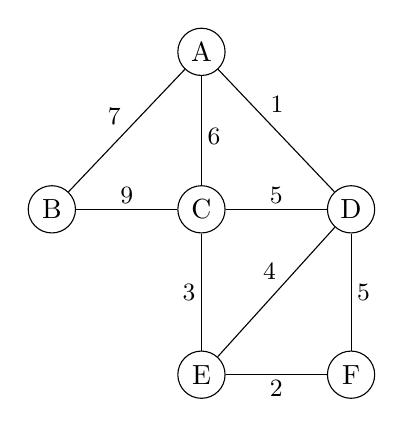
\begin{tikzpicture}[v/.style={circle,draw,minimum size=6mm,inner sep=0pt}, w/.style={font=\small,inner sep=2pt}]
\node[v] (A) at (1.9,2.0) {A};
\node[v] (B) at (0,0) {B};
\node[v] (C) at (1.9,0) {C};
\node[v] (D) at (3.8,0) {D};
\node[v] (E) at (1.9,-2.1) {E};
\node[v] (F) at (3.8,-2.1) {F};
\draw (A) -- node[w,above left] {7} (B);
\draw (A) -- node[w,right,pos=0.55] {6} (C);
\draw (A) -- node[w,above right,pos=0.4] {1} (D);
\draw (B) -- node[w,above] {9} (C);
\draw (C) -- node[w,above] {5} (D);
\draw (C) -- node[w,left] {3} (E);
\draw (D) -- node[w,above left,pos=0.45] {4} (E);
\draw (D) -- node[w,right] {5} (F);
\draw (E) -- node[w,below] {2} (F);
\end{tikzpicture}
\end{center}
\end{pastexam}

\begin{pastsoln}
答案：$1, 2, 3, 4, 7$。 最小生成樹的總權重是 $1 + 2 + 3 + 4 + 7 = 17$。

Kruskal（資結書虛擬碼~24.2）：邊依權重由小到大排，依序檢查；兩端在不同的連通塊（用互斥集合判斷）就加入，
在同一塊就跳過，因為會形成迴路。 $6$ 個頂點的生成樹有 $5$ 條邊，加滿 $5$ 條就可以停。
\begin{center}
\begin{tabular}{cclll}
\toprule
權重 & 邊 & 兩端所在的塊 & 結果 & 之後的連通塊 \\
\midrule
1 & A--D & $\{A\}$, $\{D\}$ & 加入 & $\{A, D\}$ \\
2 & E--F & $\{E\}$, $\{F\}$ & 加入 & $\{A, D\}$, $\{E, F\}$ \\
3 & C--E & $\{C\}$, $\{E, F\}$ & 加入 & $\{A, D\}$, $\{C, E, F\}$ \\
4 & D--E & $\{A, D\}$, $\{C, E, F\}$ & 加入 & $\{A, C, D, E, F\}$ \\
5 & C--D & 同一塊 & 跳過（C--E--D 已連通） & \\
5 & D--F & 同一塊 & 跳過（D--E--F 已連通） & \\
6 & A--C & 同一塊 & 跳過 & \\
7 & A--B & $\{A, C, D, E, F\}$, $\{B\}$ & 加入 & 全部連通 \\
\bottomrule
\end{tabular}
\end{center}
加入的順序是 $1, 2, 3, 4, 7$，第 $5$ 條加完就停，權重 $9$ 的 B--C 不用檢查。

兩條權重 $5$ 的邊誰先檢查都一樣，兩條都會被跳過，所以答案不受同權重順序影響。 用割性質也能確認 $7$ 一定在
樹裡：B 只連到 A（$7$）和 C（$9$），割 $\{B\}$ 上最輕的邊是 $7$（資結書定理~24.1）。
\end{pastsoln}
